\documentclass{estiloDeTesis}
\usepackage[sort]{natbib}
%\renewcommand{\bibAnnoteFile}[1]{%
%\IfFileExists{#1}{\begin{quotation}\noindent\texts c{Key:} #1\\
%\textsc{Annotation:}\ \input{#1}\end{quotation}}{}}
%\renewcommand{\bibAnnote}[2]{%
%\begin{quotation}\noindent\textsc{Key:} #1\\
%\textsc{Annotation:}\ #2\end{quotation}}
\usepackage[T1]{fontenc}
\usepackage{mathrsfs}
\usepackage{makeidx}
\usepackage[breaklinks=true]{hyperref}
\usepackage{breakcites}
\hypersetup{breaklinks=true,colorlinks=true,linkcolor=black,citecolor=black,urlcolor=black}
\usepackage{algorithm}
\usepackage{algorithmic}
%\floatname{algorithm}{Algoritmo}
\renewcommand{\listalgorithmname}{Lista de algoritmos}
\renewcommand{\algorithmicrequire}{\textbf{Entrada:}}
\renewcommand{\algorithmicensure}{\textbf{Salida:}}
\renewcommand{\algorithmicend}{\textbf{}}
\renewcommand{\algorithmicif}{\textbf{Si}}
\renewcommand{\algorithmicthen}{\textbf{Entonces}}
\renewcommand{\algorithmicelse}{\textbf{Else}}
\renewcommand{\algorithmicelsif}{\algorithmicelse,\ \algorithmicif}
\renewcommand{\algorithmicendif}{\textbf{Fin}\ \algorithmicif}
\renewcommand{\algorithmicfor}{\textbf{Para}}
\renewcommand{\algorithmicforall}{\textbf{For All}}
\renewcommand{\algorithmicdo}{\textbf{Hacer}}
\renewcommand{\algorithmicendfor}{\textbf{Fin}\ \algorithmicfor}
\renewcommand{\algorithmicwhile}{\textbf{Mientras}}
\renewcommand{\algorithmicendwhile}{\textbf{Fin}\ \algorithmicwhile}
\renewcommand{\algorithmicloop}{\textbf{Loop}}
\renewcommand{\algorithmicendloop}{\textbf{Fin}\ \algorithmicloop}
\renewcommand{\algorithmicrepeat}{\textbf{Repeat}}
\renewcommand{\algorithmicuntil}{\textbf{Until}}
\renewcommand{\algorithmicprint}{\textbf{Print}} 
\renewcommand{\algorithmicreturn}{\textbf{Retornar}} 
\renewcommand{\algorithmictrue}{\textbf{Verdadero }} 
\renewcommand{\algorithmicfalse}{\textbf{Falso }} 

\usepackage{pstricks}
\usepackage{url}
\usepackage{doi}
\usepackage{lscape}
\usepackage{color}
\usepackage[pdftex]{graphicx}
%\usepackage{graphicx}
\usepackage{epstopdf}
\usepackage{epsfig}
\usepackage{footnote}
\usepackage{longtable}
\usepackage{array}
\usepackage[section]{placeins}
\usepackage[margin=10pt,font=small,labelfont=bf,labelsep=endash]{caption}
\usepackage{subcaption}
\usepackage{listings}
\def\titulo{{Applying Homomorphic Encryption in the Cloud}}
\def\autor{Jes\'{u}s Antonio Soto Vel\'{a}zquez}
\def\grado{Ingeniero en Tecnolog\'{i}a de Software}
\def\matricula{1570031}
\def\fecha{14 de julio de 2015}
\def\asesor{Dra.\ Sara Elena Garza Villarreal}
\def\coasesor{Dra.\ Elisa Schaeffer}
\def\revisor{Dr.\ Sergio Fernando Alcaraz Corona}
\def\vobo{Dr.\ Arnulfo Trevi\~{n}o Cubero}
\newcommand{\pname}[1]{{\fontfamily{phv}\selectfont{#1}\fontfamily{cmr}\selectfont}}
\renewcommand{\lstlistingname}{Code Snippet} 
\renewcommand{\lstlistlistingname}{List of \lstlistingname s}
\setcounter{secnumdepth}{5}
\makeindex

%Paquete para texto de color
\usepackage{color}
\definecolor{red}{rgb}{1.0,0,0}
\definecolor{blue}{rgb}{0,0,1.0}
\newcommand{\comentario}[1]{\textcolor{red}{\textbf{#1}}} %Comentarios asesor
\newcommand{\correccion}[1]{\textcolor{black}{\text{#1}}} %Correcciones alumno
\newcommand{\captionFigureCorrection}{\vspace*{-6mm}}
\newcommand{\captionSubfigureCorrection}{\vspace*{-5mm}}
%\renewcommand{\tablename}{Cuadro}
%\usepackage{ulem}
\usepackage{hhline}

\makeglossary
\makeindex

\begin{document}

\frontmatter
\pagestyle{main}
\def\uanl{Universidad Aut\'{o}noma de Nuevo Le\'{o}n}
\def\fime{Facultad de Ingenier\'{\i}a Mec\'{a}nica y El\'{e}ctrica}
\def\depg{Divisi\'{o}n de Estudios de Licenciatura}
\def\snnl{San Nicol\'{a}s de los Garza, Nuevo Le�n}
\thispagestyle{empty}

\begin{scshape}
\begin{center}
	{\Large \uanl} \\[6mm]
	{\large \fime} \\[6mm]
	{\large \depg}
	\vskip 16mm
	\includegraphics[height=55mm]{uanl}
	\vskip 14mm
	\begin{tabular}{p{11cm}}
		\centering
		{\large \titulo}
	\end{tabular}
	\vskip 8mm
	{por}\\[8mm]
	{\large \autor}\\[8mm]
	{en opci\'{o}n al grado de}\\[3mm]
	{\large Ingeniero en Tecnolog\'{i}as de Software}
\end{center}

\vfill
\snnl \hfill \fecha
\end{scshape}

\newpage
\thispagestyle{empty}

\begin{scshape}
\begin{center}
	{\Large \uanl} \\[6mm]
	{\large \fime} \\[6mm]
	{\large \depg}
	\vskip 17mm
	
\includegraphics[height=50mm]{fime}
	\vskip 17mm
	\begin{tabular}{p{11cm}}
		\centering
		{\large \titulo}
	\end{tabular}
	\vskip 8mm
	{por}\\[8mm]
	{\large \autor}\\[8mm]
	{en opci\'{o}n al grado de}\\[3mm]
	{\large Ingeniero en Tecnolog\'{i}as de Software}
\end{center}

\vfill
\snnl \hfill \fecha
\end{scshape}

\newpage
\thispagestyle{empty}
\enlargethispage{5mm}

\begin{center}
{\bf \large \uanl} \\
{\bf \fime} \\
{\bf \depg}
\end{center}
\vskip 5mm

Los miembros del Comit\'{e} de Tesis recomendamos que la
Tesis \guillemotleft \titulo \guillemotright, realizada
por el alumno \autor, con n\'{u}mero de matr�cula \matricula, sea
aceptada para su defensa como opci\'{o}n al grado de Ingeniero en Tecnolog\'{i}as de Software.
\vskip 8mm

\begin{center}
El Comit\'{e} de Tesis\\          
\vskip 17mm

\begin{center}
\rule{70mm}{0.3pt}      

\vspace*{-3mm}

\asesor
\vspace*{-4mm}

Asesor
\end{center}

\vspace*{8mm}

\begin{tabular}{cc}
\rule{60mm}{0.3pt} & \rule{80mm}{0.3pt} \\
	\coasesor & \revisor \\
	Revisor & Revisor   \\
\end{tabular}

\vspace*{8mm}

\begin{center}
Vo.\ Bo.\

\vspace*{6mm}

\rule{60mm}{0.3pt}      

\vspace*{-6mm}

\vobo

\vspace*{-3mm}

\depg
\end{center}

\vfill

\snnl, \fecha

\end{center}

\chapter*{Acknowledgements}

I would like to thank all the people who made this dissertation possible, starting with my wonderful professors in the Faculty of Mechanic and Electrical Engineering at Autonomous University of Nuevo Le\'{o}n. 

Dr. Sara Elena Garza, who was both my committee chair and my first programming professor, has been of great influence towards my education on software engineering. From start to finish, she has shown great patience and never once gave up on me. She has always been a great source of motivation, helping me pull through both the classes I have taken under her, and also the projects I have collaborated with her. Whenever I strayed from my goals, her encouragement and positive attitude helped me get back in track. 

Dr. Elisa Schaeffer has always provided me with sound advice and inspiration, despite not having taking classes under her officially. The conversations I have held with her showed her passion towards the topics she teaches, which prompted me to become more engaged with other topics I was not familiar with. Dr. Sergio Alcaraz has been an invaluable professor for my education, and I greatly appreciate his patience and seriousness towards all the questions I asked during class. I had never before met a professor who seemed as pleased as he did whenever I asked questions, which motivated me to learn more of the subject and become engaged in his lectures. Dr. Iris Mart\'{i}nez and Dr. Preethy Rajesh are both amazing professors who have demonstrated that high quality education and kindness are not mutually exclusive. Finally, I would like to thank my professors from my student exchange at University of Ottawa during autumn 2012. Dr. Carlisle Adams introduced me to the world of cryptography, and because of his passion towards the subject, I became truly interested in learning about it, in spite of how complex it seemed.

My friends from Monterrey and Obreg\'{o}n city have provided me with the moral support I needed when I was writing my dissertation. I truly appreciate their kind words when I needed them the most, and also the brief distractions that helped me regain my perspective. In particular, I would like to thank Cassandra Delgado, Leticia Neaves, Alexis Rodr\'{i}guez, Luis Cano, Alan Ch\'{a}vez, Eduardo Villalobos, \'{E}rika Tapia, Marian Ju\'{a}rez, and Emilie Angel.

Finally, I would like to thank my family for their inconditional support, even as we are apart. Particularly, to my mother and role model Celia Vel\'{a}zquez, who throughout my life has supported me in all of my life goals and projects. 

\newpage

\chapter{Abstract}
\markboth{Resumen}{}

\noindent\autor.

\noindent Candidato para el grado de \grado.
%\indent 

\noindent\uanl.\\
\noindent\fime.

\noindent T\'{\i}tulo del estudio: 

\begin{center}
\begin{tabular}{p{11cm}}
	\centering
	\scshape{\large{\titulo}}
\end{tabular}
\end{center}\bigskip

\noindent N\'{u}mero de p\'{a}ginas: \pageref{lastpage}.

\paragraph{Objetives and Study Method}
%Problem
This work proposes an implementation of a client-server architecture based software that uses HElib to enable homomorphic encryption and perform computations on the encrypted data. Cloud computing is a cost-efficient alternative to host data remotely and subsequently perform computations on it. Confidentiality becomes an issue when data is delegated to the cloud, as often the information hosted is considered to be sensitive. A typical approach is to make use of a cryptographic algorithm that encrypts the data with a secret key that only the owner has. However, as long as the owner of the data wishes to make changes to the encrypted data, he would have to download the encrypted data, decrypt it using his secret key, perform the desired computations or changes to it, and reencrypt it once again before uploading it to the server in the cloud. An alternative to this approach is to make use of \emph{homomorphic encryption}, an advanced technique in cryptography that enables computations on encrypted data without needing the secret key. 

%Motivation
The motivation behind using homomorphic encryption instead of employing the typical approach is that it would not require that the encrypted data is decrypted prior to its modification, as well as it would not have to be reencrypted before uploading to the cloud, saving processing time and bandwidth. However, so far the schemes that make this possible have been thought of as being too slow and expensive, storage wise. A library that implements homomorphic encryption, HElib, is based off an homomorphic encryption scheme that seems very promising because of the optimizations and improvements over other past schemes. Using HELib, it would be possible to reevaluate the situation and show to what degree it would be feasible to make a solution based on homomorphic encryption. Therefore, it is worthwhile to make an effort to put this library into practice and measure how its use fares in a real application.

%Lo que proponemos
The proposed solution consists in taking the functionalities provided by HElib, and build a client-server based software that aims to address the main scenarios found in the proposed case study. Even though the proposed implementation could in theory work for a number of examples, it is designed taking into account a case study; therefore, both are closely related.

%Caso de Estudio
Regarding our case study, consider the scenario where a household has an expected pattern of activity, i.e. empty during the day and non-empty at night, so that the householder seeks to ascertain the number of people inside at any point in time during the day. Assuming the householder has put in place certain sensors around the building so that it detects and counts who comes in and out, he would like to learn the value of the counter remotely. As the householder chooses to store the value in the cloud, he quickly realizes he does not want others to learn of this value, not even the cloud service itself, as to prevent potential burglars to break in when the household is empty. Additionally, he wishes that the counter gets updated at certain intervals, e.g. every 20 minutes. 

%Problematica al encriptar cada vez
As it was briefly mentioned, a problem found the usual approach of re-encrypting and reuploading the data every time a change is made, is that the overhead costs might be too high to do this often. For one, bandwidth would be spent on each ocassion, and the time required for encryption and uploading might not be that short. Therefore, for this particular case study, an approach that relies on homomorphic encryption is chosen.

\paragraph{Contributions and Conclusions}
%Diferencia de los demas trabajos
In contrast with other works, the proposed solution tackles the problem by employing homomorphic encryption. It is a simple client-server architecture which could be expanded to adapt with other scenarios and requirements. The proof of concept provides the means to operate on the encrypted data, i.e. performing additions on the counter value, without compromising confidentiality and wasting resources caused by the overhead costs of re-encrypting data at every change.

%Experimentos

To show the feasibility of using HElib to do homomorphic encryption, experiments were designed by varying the value of a security parameter $k$. This value has a direct impact on the execution time of key generation, encryption, and decryption, as well as the size of the resulting public key. The findings show that even though key generation time is long, taking approximately between 9 and 13 seconds, and key size is large, being between 35 megabytes and 165 megabytes, it is not considered to be an issue, as this step is done one time only. On the other hand, encryption, decryption, and addition times are amazingly fast, none of them exceding over 1 second. However, the ciphertext raises some doubts over the magnitude of its size: during development, it was found that on average, ciphertext size was 74 megabytes; meanwhile, during experimentation, it was found that ciphertext size rose no higher than 45kB. To the best of our knowledge, there is yet no way to predict the size of the ciphertext by using HElib. Therefore, if it were found to keep the size of the ciphertext below 45kB, it would certainly be feasible to take this solution as an application on the cloud; otherwise, further evaluation on the imapct it has would be required.

\noindent Signature of Advisor: \rule{72mm}{0.3pt}

\vspace*{-4mm}

\noindent \phantom{Advisor signature: m} \asesor


\tableofcontents
\listoffigures
\listoftables
\lstlistoflistings

%\pagestyle{nom}
%\renewcommand\nomname{\'{\I}ndice de cuadros}
%\makenomenclature
%\printnomenclature[1in]
\clearpage
\pagestyle{main}
\newpage
%\printglossary
\mainmatter
\pagestyle{fime}
%%Aqui van tus abreviaciones
\nomenclature{NN}{Neural Network}
\nomenclature{HMM}{Hidden Markov Model}
\nomenclature{RGB}{Red Green Blue}
\newpage



% AQUI
\chapter{Introduction}
\label{intro}

Communication has always been a basic human need, and the means to do it is especially linked to the available technology. Thanks to the advances in techonology, it has become more common to exchange information with our peers remotely. Whether it is our personal information or current location, there are many scenarios where it is necessary to pass that information to another point. It becomes an issue when the information is considered to be \emph{sensitive}, and thus, the confidentiality of it must be protected, so that no one other than the sender and the intended receiver get to learn about the sensitive information. The medium used by both the sender and receiver to transmit any piece of information is called a \emph{channel}, which is often considered to be unsecure. It is assumed that apart from the sender and receiver, there might be a third party that tries to eavesdrop on the communication lines. In this case, it becomes important to protect the confidentiality of the information shared between the sender and receiver. 

For the scenarios where confidentiality becomes important, \emph{cryptography} becomes an attractive solution, so that encryption techniques are used to put the information in some kind of a \emph{safe}, preventing any eavesdropper to learn of its contents. The issue at hand becomes even more interesting when the safe containing the private information does not go directly to the intended party, but is rather stored somewhere in the cloud, i.e. the Internet. As long as the proper encryption mechanisms are put in place, the confidentiality is not necessarily compromised if the data were stored in the cloud. However, merely storing static information is not quite interesting: one would want to modify it as the need arises, such as when updating personal data. Such goal calls for \emph{homomorphic encryption}, which is an advanced technique used to modify the already encrypted data without compromising its confidentiality.

There are many instances where it is required to send information to someone else. To sign up for a service, for instance, several pieces of information are required. Usually, name and email address are required as basic pieces of information. Depending on the service, telephone number and personal address might also be required. In this case, the subscriber might actually be worried about how safe his information is being kept. He would feel safer if he had some kind of proof that vouched for the confidentiality of his data. This also affects the service, as less people would sign up for the service if they had no means to protect the data. There are several approaches to protect sensitive data, and one of the most effective ones is based on cryptography.

Cryptography is the study of techniques that enable secret communication, such as ciphers, that is, encryption and decryption algorithms to be used on sensitive data. Commonly, these algorithms are used to protect the data from eavesdroppers that try to pry on it. Ciphers can be seen as the means of putting sensitive data into a box with a lock, and only those with the appropriate secret key are able to access the contents of the box. It becomes troublesome to manage the secret key, because once it has been found by someone, any piece of data encrypted with the same lock becomes vulnerable to unauthorized access. Often, there is also a secure channel that is mostly dedicated to the exchange of secret keys; however, it is often limited and has certain constraints that makes it unfeasible to use it for anything else.

It has become increasingly common to delegate computing tasks to cloud services in order to save resources. For instance, these services might be used when it cannot be afforded to build and maintain a data center for the storage and computing needs that an investor might have. This is especially the case when the level of activity is seasonal: this is, requiring more processing and storage capabilities than usual during certain periods of the year. Therefore, a common solution is to make use of cloud storage and computing services, so that the costs only increase during these usage peaks. This way, the budget is spent as much as the resources are being employed, while saving configuration and maintenance costs. However, as Srinivasan \cite{Srinivasan:2012:SCC:2345396.2345474} points out, allowing the cloud service to make use of the data has raised concerns on security, since it is hard to trust that the cloud provider will not look at the data and do something with it.

A typical solution to this scenario consists in encrypting the data before storing it in the cloud; therefore, assuring its confidentiality. It is a great solution when it is only needed to read the data, without actually making any changes on it. In order to view the encrypted data, it has to be downloaded and decrypted using the proper secret key. However, when it is required to modify the encrypted data in some way, it requires to be downloaded and decrypted back to its plaintext form, before modifying it. Once it has been modified, the data has to be re-encrypted and re-uploaded to the cloud, in a potentially slow manner, depending on the size of the data. Abadi \cite{abadi2009data} explains that this approach turns out to have high overhead costs caused by the transfer of the encrypted data back and forth between the user and the cloud. In other words, it is very bandwidth intensive to encrypt and decrypt complete tables or columns out of the cloud every time some kind of change or analysis must be performed.

In scenarios where the information is not considered to be sensitive, it would be appropriate to make use of cloud computing services directly, as it would cause no harm to grant access to the data that is to be used if it were to be considered public. However, real life applications often imply sensitive data, and it should not be handled trivially, as there is no telling what kind of use an eavesdropper might give to the data.

A simple sounding, yet complicated solution to this problem would be to manipulate the encrypted data in some way such that the contents are not revealed, but on decryption, ends up being correct. In other words, to perform some kind of computation on the encrypted data, even if the private key is not known, so that when it is decrypted, the change is taken into account and the result is the same as if the operation had been performed on plaintext data. For some time, it had been thought that doing something like that was not possible, as ciphers often consisted of permutations and substitutions. However, Rivest et al. \cite{rivest1978data} noted an interesting property found in the public-key RSA algorithm (named after its creators) that proved otherwise. Such property is called ``homomorphic'', and has since then gone through a lot of research, resulting in many schemes such as ElGamal \cite{ElGamal:1985:PKC:19478.19480}, Goldwasser---Micali \cite{Goldwasser:1982:PEA:800070.802212}, Benaloh \cite{benaloh1994dense}, Paillier \cite{Paillier:1999:PCB:1756123.1756146}, among others.

\section{Problem Definition}

Even though there are many homomorphic encryption schemes that have been created to allow for computations on encrypted data, so far, they are not considered fast enough to build efficient secure cloud computing solutions. In recent years, a couple of homomorphic cryptosystems implementations have surfaced, namely: HElib \cite{helib} and FHEW \cite{fhew}. However, they are best thought of low-level building blocks for homomorphic encryption. Even though both implementations are based off optimized versions of the proposed homomorphic schemes by Brakerski et al. \cite{cryptoeprint:2011:277} and Ducas and Micciancio \cite{fhew} respectively, there have not been attempts to use these libraries to build solutions in cloud computing. As such, it has not been shown if with current implementations it is still unfeasible to build a software solution using a homomorphic scheme. In this case, feasibility is put in terms of processing time and required storage size. 

\section{Motivation}

P{\"o}tzelsberger \cite{potzelsberger2013kv} reports that there are many areas in which homomorphic encryption could be used, such as the medical, marketing, and financial fields. Until now, there was no way to make a concrete implementation of a solution related to these areas, since available schemes were either too limited or too slow. Using HELib, a library that provides fully homomorphic encryption, it would be possible to reevaluate the situation and show to what degree it would be feasible to make a solution based on homomorphic encryption.

The proposed solution consists in taking the functionalities provided by HElib, and build a client-server based software that aims to address the main scenarios found in the proposed case study. It is better thought of as proof of concept that shows how homomorphic encryption can be used in an environment that emulates cloud computing. On this attempt, basic communication functionalities are explored, as well as the flow in which the tasks are divided between the client and the server. Particular attention is put on the performance of this application, notably execution time of the homomorphic evaluations, as well as the storage required for certain items.

The idea behind this attempt is that by showing a compelling example of how homomorphic encryption can be applied in a simple scenario, cloud service providers and developers might start considering how to apply homomorphic encryption in other ways and mediums, and thus, expanding on software that makes use of it.

\section{Hypothesis}

Building a client-server based solution using the homomorphic encryption functionalities provided by HElib is feasible in terms of processing time.

\section{Objectives}

\paragraph{General Objective}

Develop a client-server based solution using HElib to perform homomorphic evaluations on encrypted data.

\paragraph{Specific Objectives}
\begin{enumerate}
\item Establish a client-server architecture where homomorphic encryption can be applied.
\item Identify which factors pose a challenge to deem applications of homomorphic encryption as inefficient.
\item Show the use of HElib to setup, encrypt, and decrypt as simple as can be.
\item Collect performance data on the use of homomorphic encryption.
\end{enumerate}

\section{Case study}

Consider the scenario where a household has an expected pattern of activity, i.e. empty during the day and non-empty at night, so that the householder seeks to ascertain the number of people inside at any point in time during the day. Assuming the householder has put in place certain sensors around the building so that it detects and counts who comes in and out, he would like to learn the value of the counter remotely. As the householder chooses to store the value in the cloud, he quickly realizes he does not want others to learn of this value, not even the cloud service itself, as to prevent potential burglars to break in when the household is empty. Additionally, he wishes that the counter gets updated at certain intervals, e.g. every 20 minutes. 

A typical approach consists in encrypting the counter value every time it is recalculated, replacing the older value stored in the cloud server. Considering the overhead costs of this process, he considers another potential approach that makes use of homomorphic encryption. The sought solution needs to eliminate the need to reupload the counter value every time it is updated by a change in the number of people in the household. Additionally, the private key should only be in the possession of the householder, so that even the cloud hosting service does not have the ability to learn the value of the counter. Finally, whenever he needs to know of the current value of the counter, he can download the encrypted value and, using the previously generated secret key, decrypt the data to obtain the value of the counter.

\section{Structure}
This thesis is made up of the following chapters: introduction, background, related works, methodology, experiments, experiments and results, and conclusions.

In this chapter, both the problem definition and motivation were posed to build a client-server architecture using HElib to address the scenario of the proposed case study.

In Chapter \ref{background}, necessary basic notation and definition of concepts on cryptography are presented to acquaint the reader with the content presented in the thesis.

Chapter \ref{relatedWorks} presents some works that are related to solutions based on homomorphic encryptography. The characteristics of each work is briefly described and compared with the ones presented in this thesis.

Chapter \ref{methodology} presents the implementation details of the proposed client-server architecture, describing each component and how the functionalities of HElib are put in use. Additionally, the case study is addressed within the scope of the client-server solution as well.

Chapter \ref{results} presents the performed experiments to test certain parts of the client-server implementation related to the use of homomorphic encryption, as well as showing the results pertaining to the processing times and size. Afterwards, it presents conclusions based on these results.

Finally, Chapter \ref{conclusions} presents general conclusions obtained from the results during the experimentation phase. Aditionally, some recommendations regarding the implementation of the client-server architecture are presented to be considered as future work.

\clearpage

\chapter{Background}
\label{background}

\textbf{Information Security and Data Confidentiality}

Information security is a broad topic that covers many different aspects, from which two of them are particularly important for this work: confidentiality and authentication. There are some aspects from cryptography that would be relevant to review, such as asymmetric and symmetric cryptography, as well as the concepts: plaintext, ciphertext and key. A brief description of cloud computing and its relevant aspects are to be described, and how can secure computations have an impact on it. Finally, the concept of homomorphic encryption will be explained, noting the mathematical properties and its categories of somewhat homomorphic encryption and fully homomorphic encryption.

Seen from a general perspective, Whitman and Herbert describe security as ``the quality or state of being secure---to be free from danger'' \cite{PrinciplesInformationSecurity}. Danger would refer to a potential harming action that an adversary can do, whether it is intentionally or not. Computer security is defined by the NIST Computer Security Handbook as follows:

``The protection afforded to an automated information system in order to attain the applicable objectives of preserving the integrity, availability, and confidentiality of information system resources (includes hardware, software, firmware, information/data, and telecommunications)''.

This definition introduces two relevant concepts in the previous definition, namely: information and confidentiality. RFC 2828 defines information as ``facts and ideas, whichcan be represented (encoded) as various forms of data,'' and data as ``information in a specific physical representation, usually a sequence of symbols that have meaning: especially a representation of information that can be processed or produced by a computer.'' Although both terms have different connotations depending on what it represents, both words are used interchangeably in this work. Now that information has been described as a concept, confidentiality can be introduced. More specifically, data confidentiality refers to the assurance that private or confidential information is not made available or disclosed to unauthorized individuals \cite{CryptoStallings}. This term is closely related to \textit{privacy}, which gives individuals the control of what information related to them may be accessed or stored by whom. Loss of confidentiality would imply unathorized access or disclosure of information.

\textbf{Cryptography Concepts}

Cryptography is the study of protecting data and communications. It involves communicating messages or information between two or more parties by changing the appearance of the messages, so that it becomes very difficult for unauthorized parties to intercept or interfere with the transmission of the information \cite{IntroCryptoMath}. Cryptography should not be confused with cryptology, because even though they overlap with each other, cryptology includes cryptanalysis as well. 

Other important aspects that have been linked to cryptography apart from confidentiality are \textit{authentication} and \textit{integrity}. Authentication gives the receiving parties the means to make sure that the source of the communication is really who it is thought to be, and not someone pretending to be the legitimate sender. On the other hand, integrity, among other things, ensures that the message received has not been tampered in any way. Different kind of cryptographic algorithms are required to satisfy these goals, and the same goes for confidentiality.

\cite{CryptoIT} approaches the study of cryptography by explaning the classical problem of transmitting secret messages from a sender A to a receiver B. Both the sender and receivers, A and B, can be thought of persons, organizations, or various technical systems.  They are formally described as abstract ``parties'' or ``entities'', but it is often more convenient to identify both of them as human participants that go by the names of Alice and Bob, instead of using the letters A and B.
For the messages to go from Alice to Bob, there has to be some kind of medium or channel where the information is transmitted. Generally, it is assumed that the channel can be potentially accessed by a third party that is neither the sender nor the receiver. On top of it, it is also assumed that either the receiver or sender has an adversary or enemy E, who is constantly trying to tamper or know the content of the messages passed between Alice and Bob. This attacker E who is constantly eavesdropping on the communication lines is usually called Eve, who is thought to have powerful computing facilities and is able to make use methods to learn of the message contents.  It is clear that both Alice and Bob want to protect their messages so that their contents are unclear to Eve. This implies a confidentiality goal, and it can be reached by using encryption algorithms, or as they are commonly known: ciphers.
Before a message is sent from Alice to Bob or viceversa, the sender \textit{encrypts} the message. In other words, a certain algorithm is applied on the message so that the content of it is unclear to a third party, such as Eve. Once the sent message has been received by the other party, he \textit{decrypts} it to recover the original content of the message before encryption, known as \textit{plaintext}. In order for this to work, Alice and Bob must have agreed in advance about various of the details needed, such as the algorithm and parameters used by the sender, so that the receiver knows how to perform the decryption properly. Since it would be troublesome that Eve learned of those details, Alice and Bob would have to use some sort of secure channel, such as trusted messngers or couriers, or set up a private meeting where no one else can eavesdrop. Making use of this secure channel, however, is more costly than using the regular communication channel between Alice and Bob, and it might not be available at all times, which is why it is recommended to use it only to agree on some details in advance, like the parameters for the encryption algorithm, as well as a \textit{private key}.
As Stanoyevitch \cite{IntroCryptoMath} describes it on his Introduction to Cryptography book, the above scheme would make up a cryptosystem, since it makes of cryptographic algorithms. As it has been hinted, such a cryptosystem has two parts: encryption, which is done by the sender as means of putting or transforming the actual \textbf{plaintext} into \textbf{ciphertext}, and \textbf{decryption}, which is done once the message has been received at the other end and has the purpose of translating the ciphertext back into the original plaintext message. Both encryption and decryption are usually done using a \textbf{key}, and it is intended that only the sender and receiver learn of the nature and value of the key. 

[INSERT BOB-ALICE-EVE DRAWING]

The use of the plaintext, ciphertext, and key concepts are recurrent throughout this work, and given their relevance, they are explained as follows, along with other concepts, the same way Cameron \cite{CryptoNotes} and Stallings \cite{CryptoStallings} describe them.
\begin{description}
\item[Plaintext] It is the original message that Alice wants to send to Bob. Neither Bob nor Alice want the message to be known to Eve. This piece of data is fed into the encryption algorithm before it is sent to the other end.
\item[Encryption algorithm] This algorithm uses a key that performs several substitutions and transformations on the plaintext. The result is a ciphertext that cannot be translated back to its original plaintext form without the appropriate key.
\item[Secret key] It is a value that both Alice and Bob agree upon, it is usually kept secret, since it is used by the encryption algorithm to obtain the ciphertext. The encryption algorithm will produce a distinct output depending on the key being used. In other words, if the secret key is leaked to Eve, this would mean that Eve can now learn any messages that are being produced using that key.
\item[Ciphertext] This is the modified or scrambled message produced as output by the encryption algorithm. Its value depends on the algorithm and plaintext, as well as the chosen key.
\item[Decryption algorithm] It is like the encryption algorithm, except that its run in reverse. The has two inputs: the ciphertext and its corresponding key. It then performs the necessary substitutions and transpositions so that the ciphertext is translated back into the original plaintext.
\end{description}

It is assumed at all times that Eve has access to the communication lines, and can always know the ciphertext that is being sent between Alice and Bob. It is also a good practice to assume that the encryption and decryption algorithms are known to Eve, which leaves the key as the most important part of the scheme. As mentioned previously, Alice and Bob need to establish the means to to agree on a private key, without anyone else knowing what this key is. As soon as the key is known to the attacker, i.e. Eve, all further communication is compromised. When that happens, another key has to be chosen and agreed upon once more by Alice and Bob.

The nature of the encryption and decryption can be classified in two broad categories: symmetric and asymmetric key encryption. \cite{CryptoKeys} describes both categories by looking at the keys used. In \textbf{symmetric encryption}, the key used for encryption is virtually the same used in decryption. Therefore, key distribution has to be done before the tranmission of the messages. The key length has a direct impact on the security offered by the encryption algorithm. Meanwhile, \textbf{asymmetric encryption} employs two different keys: public and private. The public key is closely tied to the receiver, and it is used for encryption of the data. It is called public because it is available for general use; therefore, Alice can use Bob's public key to send him messages. On the other hand, the private is kept secret from the outside world, and is only available by an authorized person. The public and private keys always come in pairs, and this is because while the public key is used to encrypt data; its counterpart, the private key, is used to decrypt the data. 

\textbf{Number theory: Groups, Rings}


\textbf{Services in the cloud}

The cloud, a trendy term used to describe a network of servers usually accessible through the Internet, currently provides two important services: storage and computation. As Xu et al. in \cite{cryptoeprint:2011:574} point out, cloud storage services, such as Dropbox, Skydrive, Google Drive, and Amazon S3 have become very popular in recent years. As the use of these services become more common, more sensitive information is kept in the cloud, such as emails, health records, private videos and photos, company finance data, government documents, etc. 

Li, Jin et. al \cite{cryptoeprint:2009:593} introduce cloud computing as a new term that views computing as an utility which enables convenient, on-demand access to computing resources that can be rapidly deployed with minimal management overhead and great efficiency. Cloud computing has the potential to benefit its users in avoiding large capital expenditure used for deployment and management of both software and hardware, such as setting up a data center. 

All of these services are opening up a new era powered by the software as a service (SaaS) computing architecture. One of the main advantages of storing this information in the cloud is that the owners are relieved from the burden of data storage and maintenance at all times. There are many plans that adjust to the on-demand needs of the owner of the data, which is way less costly than building and maintaining a whole data center. This implies that the clients of these services can expect to gain reliability and availability from having the data stored remotely. On the other hand, the data is necessarily brought out of their control and protectio. This becomes a risk for the owner of the data, since the information stored in the cloud could potentially be accessed by unauthorized individuals, such as competitors or malicious attackers. There also exists the possibility that the information stored could be tampered in some way, thus compromising its integrity. Therefore, the computing and storage service providers are usually not trusted completely, which is why it has been difficult for the public and organizations to fully adopt the use of these services.

The aforementioned issue brings up the need of having a mechanism that verifies that a cloud provider is storing the whole database intact, even the portions that are rarely accessed. Ateniese et al. \cite{cryptoeprint:2014:886} point out that, fortunately, a series of \textit{proofs-of-storage} protocols have been proposed to solve this problem related to data integrity. Xu et al. \cite{cryptoeprint:2014:395} define a proof of storage (POR or PDP) as a cryptographic tool, which enables a data owner or third party auditor to audit integrity of data stored remotely in a cloud storage server, without keeping a local copy of data or downloading data back during auditing. In other words, applying a proof of storage in a cloud server can guarantee that the data has not been tampered with; and in the event that it is, most likely the service could be held liable for damages to the data. A huge advantage of using a proof of storage is that the data does not have to be downloaded to confirm its integrity, which makes it ideal to make use of it routinely. 

One of the simplest use cases for cloud computing is when a user independent from the cloud wants to store some data in it for later retrieval. In this simple case, data confidentiality and integrity can be trivially ensured. For that, typical cryptography primitives can be usedby encrypting the user's data before it is sent for storage in the cloud. To ensure confidentiality, the key used for encryption is kept secret from the cloud provider. However, real life applications are not as simple. Damgard et al. \cite{cryptoeprint:2013:629} mentions that the cloud is more than a storage medium; in particular, computation over the stored data is outsourced to the cloud. Sometimes it might even be distributed among distinct cloud servers geographically apart, operated by different parties. Wang et al \cite{cryptoeprint:2009:081} describe the nature of the problem at length, because usually a cloud service is not solely restricted as a data warehouse. The data stored in the cloud may be frequently updated by the users, including insertion, deletion, modification, appending, reordering, etc. This kind of complex scenario is what makes the use of traditional cryptographic primitives so difficult to adapt, especially because the data is not stored in a single cloud server, but is instead redundantly stored in multiple physical locations to further reduce the data integrity threats. Therefore, making use of cloud services highly improve data avalability and storage flexibility, data confidentiality and integrity is put at risk.


\textit{Key management}

\textbf{Secure multiparty computation}

\textbf{Homomorphic Encryption}

\textit{Intro}

\textit{Mathematical things}

According to P{\"o}tzelsberger \cite{potzelsberger2013kv},  \textit{homomorphic cryptosystem} is a cryptosystem whose encryption function is a homomorphism, and thus preserves group operations performed on ciphertexts. Arithmetic addition and multiplication are the two group operations considered.  A homomorphic encryption is additive if:

\begin{equation}
\epsilon(x+y) = \epsilon(x)\otimes \epsilon(y)
\end{equation}

where \epsilon denotes an encryption function, \otimes denotes an operation depending the used cipher and x and y are plaintext messages. A homomorphic encryption is multiplicative if:

\begin{equation}
\epsilon(x \cdot y) = \epsilon(x) \otimes \epsilon(y)
\end{equation}

where again \epsilon denotes an encryption function, \otimes denotes an operation depending on the used cipher and x and y are plaintext messages.

\textit{Classification}

Homomorphic encryption schemes are classified in two broad groups


\textit{Applications}

\textit{Intro to lattice-based crypto}

\textit{BGV scheme}



\clearpage

\chapter{Related Works}
\label{relatedWorks}

Pending ....
%En este cap\'{\i}tulo se presentan cuatro trabajos relacionados con el sistema de detecci\'{o}n de reportes duplicados desarrollado en esta tesis. Se realiza una breve descripci\'{o}n de cada uno de los trabajos y se explican las similitudes y diferencias entre esos trabajos y este trabajo de tesis.

\clearpage

\chapter{Methodology}
\label{methodology}

This work looks at a case study which presents an issue directly related to the confidentiality of information when it is being stored in the cloud. It discusses the situation where it is important to be able securely store a secret value, as well as make modifications on it. A solution to the problem is proposed by employing homomorphic encryption. Then, it describes in a general way a proof of concept as a stand-alone solution. Afterwards, the scenario of using a client-server architecture is considered, discussing some decisions that were made regarding the communication needs. Relevant points on key management are mentioned, and also, how the tasks previously mentioned are being split by each component. 

The methodology in this work describes all the considerations and steps taken to build a solution to the problem analyzed from the case study. As such, the methodology has a very close relationship with the case study. Even though the object of study is the application of homomorphic encryption in the cloud, it is not trivial to find a fitting situation where it can be applied. The search becomes more complex as the limitations of state-of-the-art homomorphic encryption tools are considered. The case study that was thought of is simple enough so that the currently available tools can be used effectively, and complex enough so that applying homomorphic encryption is compelling and better than other alternatives.

\textbf{Case study}

The case study is explained as follows: a household commonly has more than one member, e.g. partner and children. The responsible members of the household (i.e. the parents) might want to keep an eye on the house while being away, especially if children are left behind. They would like to ensure that their children stay inside during this time, and that nobody else, except for a babysitter, enters the house. And if it were the case that somebody got in or out, they would probably wish to be promptly notified of it. This is especially true for the case when they are away for long periods of time, during a vacation, for example. A traditional solution consists in setting up a surveillance system throughout the house, which would certainly work to prevent robbery, but wouldn't necessarily work as a measure to know whether or not the children have left the house. Setting a surveillance system might be too costly for some families, and not be quite adaptive to their needs. It might be more efficient to deploy a system that detects when people enter and exit the building through the main door, and keep a counter of it. The main idea is that the \textit{surveillance count} gets initialized at some point in time, and, as people go in and out, the counter increases or decreases, respectively. Setting up the sensors and other pieces of hardware can be considered as a Do-It-Yourself project, as resources could easily be found. The issue comes out when the recorded data, that is, the counter, is to be accessed remotely via some kind of web application. 

[INSERT SAMPLE FIGURE]
% pendiente poner imagen

\textbf{Proposed solution}

The proposed solution addresses the issue hinted at the end of the study case description. This refers to making available the counter data to the householder without compromising confidentiality. Assuming that there might be more than one person who would have access to this data per household, it might not be appropriate to set up a Peer to Peer communication scheme. It makes more sense to have a server in the cloud that stores the counter data, waiting for requests from the clients to deliver the information. The data stored in the server is to be accessed from anywhere else; however, one of the most important aspects of the whole scheme remains unaddressed: confidentiality.

Usually, the householder would not allow others to know about the actual counter, including the server, as this information is considered to be sensitive. The traditional approach is to make use of public-key cryptography to encrypt the data and prevent from anybody else to know the counter. The counter value would then have to be encrypted using a certain cipher before it is uploaded to the cloud. However, this would imply that every time that there is a change in the counter, the whole ciphertext would have to be reuploaded to the server. Considering that person comes in and out of a building quite frequently, it would turn out to be a heavy burden which has an overhead cost that keeps accumulating every time there is an update. 

An alternative approach is to simply notify the cloud service of any changes that occur, so that it performs the addition or subtraction itself instead of relying on receiving the whole encrypted result. Even though this would not be possible to do with traditional cryptography, it can be done using homomorphic cryptography. The concept behind this approach is that, while initial counter value is being stored on the server, the client part that resides on the household sends over any change of individuals that are inside the building, and so the cloud service, i.e. the server, performs the appropriate homomorphic computations on the currently stored value. This occurs without the need of anybody reuploading the counter data again, and the server has no need of decrypting the data in the first place. Since the full ciphertext is not being resent, the overhead cost is reduced significantly.

Whenever the householder needs to know the value of the counter, he can authenticate with the cloud service to download the current ciphertext that represents the counter. The ciphertext can decrypted using the private key generated in the beginning. This aspect remains the same whether homomorphic encryption is used or not, and there is no way around it without compromising confidentiality. Considering that a system that detects when people come in and out might not be perfect, and if somehow the counter gets to an incorrect value, it could be reset to the correct amount. In this case, it would be unavoidable to send a newly encrypted counter value.

The solution itself consists in an implementation of a client-server software that aims to store and modify a secure counter by making use of homomorphic encryption. The various tasks that help reach this goal are distributed by the client and server components of the software. The client focuses initialization of the homomorphic encryption scheme, generation of public and private keys, encryption of initial counter data, among other things. On the other hand, the server is dedicated to store and manage the public key of the user and his current counter value. Both parts of the software utilize a library called HELib, which makes it possible to run homomorphic evaluations. In other words, this library is used perform basic operations on it, such as addition, subtraction, and multiplication. Consequently, it is also used to generate the public and private keys, encrypt data, and decrypt it. Once the encrypted counter is stored in the server, a different kind of client can then ask to download and decrypt it. It makes sense to say that it will be a different kind of client, since most likely the interested person would not be at the place where the counter was initialized.

% \textbf{Scope}

% The scope of the solution is limited to a software implementation that addresses the aspects of securely storing, modifying and accessing sensitive data on the cloud.
% These aspects include other important topics, such as key management, which is crucial for the cloud service to know which public key to use during the homomorphic operations. 

\textbf{Details of the HELib library}

An implementation of an homomorphic encryption scheme, the Brakerski-Gentry-Vaikuntanathan (BGV), is openly available as a C++ library, called HELib. Using this library, it is possible to encrypt integer values and perform operations on them while being encrypted. There are many parameters to be considered when using this implementation, and these usually define how the public and private keys are going to be like. For this particular application, most parameters were left in their default values, as they seemed to serve the purpose. 

Part of the description in the code repository of HELib, it is stated that the library is considered to be low-level, and given its difficulty and constant changes, not that appropriate to use to build big applications with it.  [quote] 'At its present state, this library is mostly meant for researchers working on HE and its uses. Also currently it is fairly low-level, and is best thought of as "assembly language for HE". That is, it provides low-level routines (set, add, multiply, shift, etc.), with as much access to optimizations as we can give.'

It is important to note that the library recently started to support multi-threading, which would considerably speed up the evaluation times of the homomorphic operations. Not too long ago it started to support bootstrapping as well, a technique that prevents the ciphertext from getting too much noise and results in the incorrect evaluation of the operations.

\textbf{Setting up the parameters and context}

The HElib library is an implementation of a homomorphic encryption scheme, and as such, it has certain requirements before it can encrypt data or even generate keys. First of all, it has a list of parameters which must be manually set. Depending on the parameters applied, some aspects that directly affect the keys and ciphertext are altered. The suggested values are used for the majority of the parameters. Altering the values of the parameters could be an interesting way to do experimentation with the key size and computation time required.

The following table briefly describes each parameter used in HElib. It does not go into much depth, as those details are mostly pertaining to the algorithms in the library.

%\begin{table}
  \begin{tabular}{|l|c|r|}
    \hline 
    R  &     number of rounds &  default=1     \\ \hline
    p  &     plaintext base  & default=2  \\ \hline
    r  &     lifting  & default=1  \\ \hline
    d  &     degree of the field extension  & default=1  \\ \hline
    c  &     number of columns in the key-switching matrices  & default=2  \\ \hline
    k  &     security parameter & default=80  \\ \hline
    L  &     number of levels in the modulus chain  & default=heuristic  \\ \hline
    s  &     minimum number of slots  & default=0  \\ \hline
    repeat &  number of times to repeat the test & default=1  \\ \hline
    m   &    use specified value as modulus & optional  \\ \hline
    mvec &   use product of the integers as  modulus & optional \\ \hline
    gens &   use specified vector of generators & optional \\ \hline
    ords  &  use specified vector of orders & optional \\ \hline
  \end{tabular}
%  \caption{Parameters used for use of HElib}
%\end{table}


\textbf{Key generation and serialization}

As this library requires the use of public and private keys, the user is required to create his own set of keys, and it is only the public key which he should be willing to share. The user then shares his public key with the cloud service by some means of registration, so he does not have to share it every time he makes use of the service. The public key is used to encrypt the counter data for the first time before sending it over to the server, and the server itself requires this public key in order to perform the homomorphic operations.
The generation of the keys is pseudorandom, so extra care should be taken as to not to use a predictable seed, so that the public and private keys are not recreated by someone else. 

After instantiating context with all the necessary parameters, the set of keys can be generated. Firstly, the public key is obtained by simply instantiating an object of the class \textit{FHESecKey}. Then, a copy of the public key is made as the foundation for the private key. This copy makes use of a method called \textit{GenSecKey(w)}, which takes \textit{w} as a seed to create the real private key. Finally, it goes through a process that computes key-switching matrices, which are used in the internal algorithms of the library.

\begin{lstlisting}
  publicKey = new FHESecKey(*context);
  secretKey = publicKey;

  secretKey->GenSecKey(w); 
  addSome1DMatrices(*secretKey); 
\end{lstlisting}

Before proceeding to encrypt the data, it is important to have the public key serialized and ready to send it to the server. Serialization is a popular term used to describe the encoding of objects and the objects reachable from them, into a string of bytes. It is commonly used for lightweight persistence and for communication via sockets 
[reference: http://docs.oracle.com/javase/8/docs/technotes/guides/serialization/index.html ]. In this case, it is used as a means of temporarily saving the public key in a stream of bytes so it can be shared with a remote server that will be able to read such stream. Only after the contents of the saved object have been fully read, it is possible to reconstruct the public key. Fortunately, the HElib provides a very simple way to do serialization, since the class 
\textit{FHESecKey} supports the \textless\textless operator which works quite nicely with a couple popular serialization class in C++ called \textit{istringstream} and \textit{ostringstream}. The use of this class is showed as follows: 


\begin{lstlisting}
  ostringstream pkstream;
  pkstream << *publicKey;
\end{lstlisting}


This way, the data of the attributes found in the public key object has been stored as a stream of bytes in a highly portable object from the \textit{ostringstream} class. Using this newly populated object, the public key can be shared using sockets.

\textbf{Encryption of the Counter Value}

In order the protect the value of the counter from being known from other parties, including the server itself, it must be encrypted. This means that an encryption algorithm, provided by the HElib, is to be used on the plaintext that represents the counter. The result of this process is a ciphertext, which, unless provided with the corresponding private key, cannot be brought back to its plaintext form. 

Following the conventions defined in the HElib, an object from the \textit{EncryptedArray} is initialized using the \textit{context} and \textit{G} which were previously set. \textit{EncryptedArray} can be seen as a container for the plaintext, where the value of the counter is placed. Once it has been done, a method called \textit{encode} of the same class can be used to prepare the data for encryption. The ciphertext is stored in a different kind of container, which comes from the class \textit{Ctxt}. This container is initialized using the public key as argument. Afterwards, the encryption of the plaintext data can be done using a method of the \textit{EncryptedArray} object simply called \textit{encrypt}. This method receives as arguments the objects of the plaintext and ciphertext containers, and the public key.

\begin{lstlisting}
  EncryptedArray ea(*context, G);
  PlaintextArray counter(ea);  
  counter.encode(people);
  Ctxt& encryptedCounter = *(new Ctxt(*publicKey));  
  ea.encrypt(encryptedCounter, *publicKey, counter); 
\end{lstlisting}

This ciphertext can be used in several ways: its value can be modified by adding, substracting or multiplying it by some arbitrary value, it could also be decrypted at any time using the private key, or it could be serialized as it was done with the public key, so another party, e.g. the server, can receive and store it.

\textbf{Single component operation flow}

Before attempting to break down the whole implementation in two parts: the server and client side, a proof of concept was implemented which combined the tasks of both parts into a single program. The flow of this program represents how the data gets transformed through several tasks. 

\begin{enumerate}
	\item Parameters to use with the HELib are arbitrarily chosen, while other required values are computed.
	\item Context of the HELib library is set.	
	\item Public and private keys are created using the context.
	\item Optionally, public key can be serialized into a file so it can be used later.
	\item The structures to store plaintext and ciphertext are declared.
	\item The initial counter value is set into the plaintext structure.
	\item The plaintext is encrypted using the public key and stored into the ciphertext structure.
	\item Values are arbitrarily added or substracted from the ciphertext.
	\item Ciphertext is decrypted using the private key, and its value is stored in another plaintext structure.
	\item Newly decrypted plaintext is printed to verify correct result from operations.
\end{enumerate}

\textbf{Software Architecture and Data transmission}

Even though the case study started out considering cloud services, an actual implementation of the application can be addressed with a client-server architecture. The client-server architecture is a popular model that consists of a two parts: a client and a server. Usually, the server just waits for any kind of request from a client to do some kind of task. Meanwhile, the client usually starts some kind of task, but depends on the server to do it completely. Most of the time, the client depends on the server because it might have something that the client does not, like a database.

In this case, the implementation of the counter application is approached using a client-server model. The server represents the cloud service that stores and modifies the encrypted data on request, while the client plays the part of obtaining and encrypting the sensitive data. The client also takes care of tasks such as initializing the homomorphic encryption context, generating the public and private keys, encrypting the data, and serializing the encrypted counter before sending it over to the server. Meanwhile, the server takes care of establishing the communication details via TCP sockets, reconstructing the received ciphertext, and performing operations on it. Although a more secure implementation would consider using the Secure Socket Layer (SSL) over TCP, it was simplified to cover only the details pertaining the use of homomorphic encryption.

Once the user has obtained the initial data, i.e. by counting the number of people currently in the house at a given time, he proceeds to feed the data to the client program, so it is encrypted using the previously generated public key. After the counter data has been encrypted successfully, the data is then sent to the server via sockets. There were two possible protocols that could have been used for this part: UDP and TCP. UDP stands for User Datagram Protocol and is used in conjunction with the Internet Protocol. UDP works best when the data units that are being sent are very small. It is also a little bit problematic considering that it does not reassembles data packets once they have arrived at the destination. The other option that was considered was TCP, which stands for Transmission Control Protocol. It is a little friendlier to use in the sense that it reassembles datagrams in the correct order once they arrive at their destination. However, it adds a little bit of overhead cost since it adds a header section per segment. In the end, it was chosen to use TCP over UDP, especially since it might become complicated to keep track of the order of the data packets.

\textbf{Sending and reading serialized data}

The serialized data that is sent through sockets was very large to be done with a single function call, which is why a few considerations have to be made on the implementation. It is recommended to have some kind of supporting function that continuously is attempting to send data to the server, until there are no bytes left.

The following snippet of code shows how the ciphertext is serialized using the \textit{ostringstream} class, and then a function call is made to a supporting function which continuously attemps to send all the remaining bytes to the server. It is relatively simple to keep track of how many bytes are being sent and how many are left, which is why it stops sending data at the appropriate time.

\begin{lstlisting}
  ostringstream oss;
  oss << encryptedCounter;

  if(sendalldata(sockfd, oss.str().c_str(), &msgsize) == -1) {
    printf("ERROR. Only \%d bytes sent!\textbackslash n", msgsize);
  }

int sendalldata(int s, char const* buffer,  int *len)
{
  int total = 0; // bytes sent
  int bytesleft = *len; // bytes left to send
  int n;
  
  while(total < *len) {
    n = send(s, buffer+total, bytesleft, 0);
    if (n == -1) { break; }
    total += n;
    bytesleft -= n;
  }
  *len = total; 
  if(n == -1) 
    return -1;
  else 
    return 0;
}
\end{lstlisting}

As it cannot be expected that the serialized ciphertext of great size will be succesfully sent with a single send function call, the same goes for the receiving end. Certain measures have to be taken so that all the data is received complete and in the appropriate order.

The following piece of code extracted from the server side of the software goes through the part where the ciphertext is being received after it has been serialized. First of all, a buffer is declared and initialized with the size of the ciphertext, which was previously received. A function called \textit{bzero()} is used to prepare and empty the buffer.  Then, a while loop is done as long as there are bytes remaining to be received. As more iterations go by, more data is appended to the buffer. A couple of variables are used to keep in check how many bytes have been read and how many are still pending to be read.

\begin{lstlisting}
  char* responseBuffer = new char[responseBufferSize];
  bzero(responseBuffer, responseBufferSize);
  bytes_read = 0;
  int bytes_remaining = responseBufferSize;
  int this_recv;
  while(bytes_remaining > 0) {    
    this_recv = recv(newsockfd, responseBuffer+bytes_read,
                bytes_remaining, 0); 
    if(this_recv <=0) error("error on receive");
    else {
      bytes_remaining -= this_recv;
      bytes_read += this_recv;
    }
  }
\end{lstlisting}

\textbf{Reconstructing the ciphertext}

It was mentioned before that serialization allowed persistence and made it easier for object data to be sent via sockets. However, the serialzied objects cannot be used the way they are received. In this case, the ciphertext was serialized before being sent to the server, and once it is properly received, the data must be used to reconstruct the original ciphertext object.
If this is not done, there is no way to perform operations on the ciphertext, or even decrypt it to know its value.

The following piece of code describes the steps to be taken in order to reconstruct the object that can contain the ciphertext. First of all, the buffer that was previously filled with data is then copied into a string variable, then it goes through a couple of steps so it can be used as a \textit{istringstream} object. The preparation is certainly more complicated, but the reconstruction of the object is quite simple itself. Since HElib is friendly with the \textgreater\textgreater operators, it can be done in one step. This operator basically takes the data from one variable and puts it in another kind of variable, one being a \textit{istringstream} object, and the other a \textit{Ctxt} object.

\begin{lstlisting}
  string strBuffer((const char*) responseBuffer, bytes_read);
  istringstream serialCipher;
  serialCipher.str(strBuffer);

  Ctxt receivedCipher(publicKey);
  serialCipher >> receivedCipher;
\end{lstlisting}


\textbf{Changes in the counter}

Once the initial value of the counter has been received by the server, there are two possible scenarios that could occur next: the value gets viewed by the householder, or a change in the counter occurs. Whenever a significant change is observed by the client program, the change is promptly notified to the server, which could be either positive or negative. When the cloud service receives the value of change, it either adds or subtracts it from the previously stored value. The change is immediately visible to the householder who might wish to know the current value of the counter.

As the implementation of the counter was started before December 2014, bootstrapping was not considered to use. Bootstrapping is an advanced technique in fully homomorphic encryption which allows more homomorphic evaluations to be run on a ciphertext. As it has been mentioned, whenever a homomorphic evaluation is performed on the ciphertext, a small amount of noise is added to it, and after a certain threshold, the ciphertext becomes unusable, in the sense that it no longer decrypts back to the correct value. As an alternative to bootstrapping, however, it is possible to reset the counter, i.e. upload a newly created ciphertext with an initial counter value, so that more homomorphic evaluations can be performed on it. Considering that the operations that will be done most of the time are addition and subtraction, this is not something that will occur often, but eventually will. 

\textbf{Architecture breakdown}

The proof of concept that makes use of homomorphic encryption ends up being completely linear in the sense that it has no communication at all with different parts of the outside world. The considered case study implies that there is both a household where the counter is initialized and another location where the current counter value can be accessed. Considering this aspect, it makes sense to have a server in the cloud that can be accessed securely which will contain the current value of the counter for each household. This requires the server to store the public key as well, since to be able to modify the ciphertext of the counter data, such a key is needed. 

In the following figure, a breakdown of the client-model architecture employed is depicted. As previously mentioned, the solution is split into two parts: client and server sides. Each side has specific tasks that must be performed independently. The figure was conceived as an attempt to organize the software structure and assign a functionality to one of the components. The client side is in charge of the tasks that are performed at the place where the counter is initialized, i.e. the household. Such tasks include: setting up the parameters and context required by the HElib, generating the set of public and private keys, registering the public key, encrypting the initial counter value, serializing the ciphertext, recording changes in the counter value, and decrypting the received ciphertext. 

\begin{figure}[h!]
  \centering 
  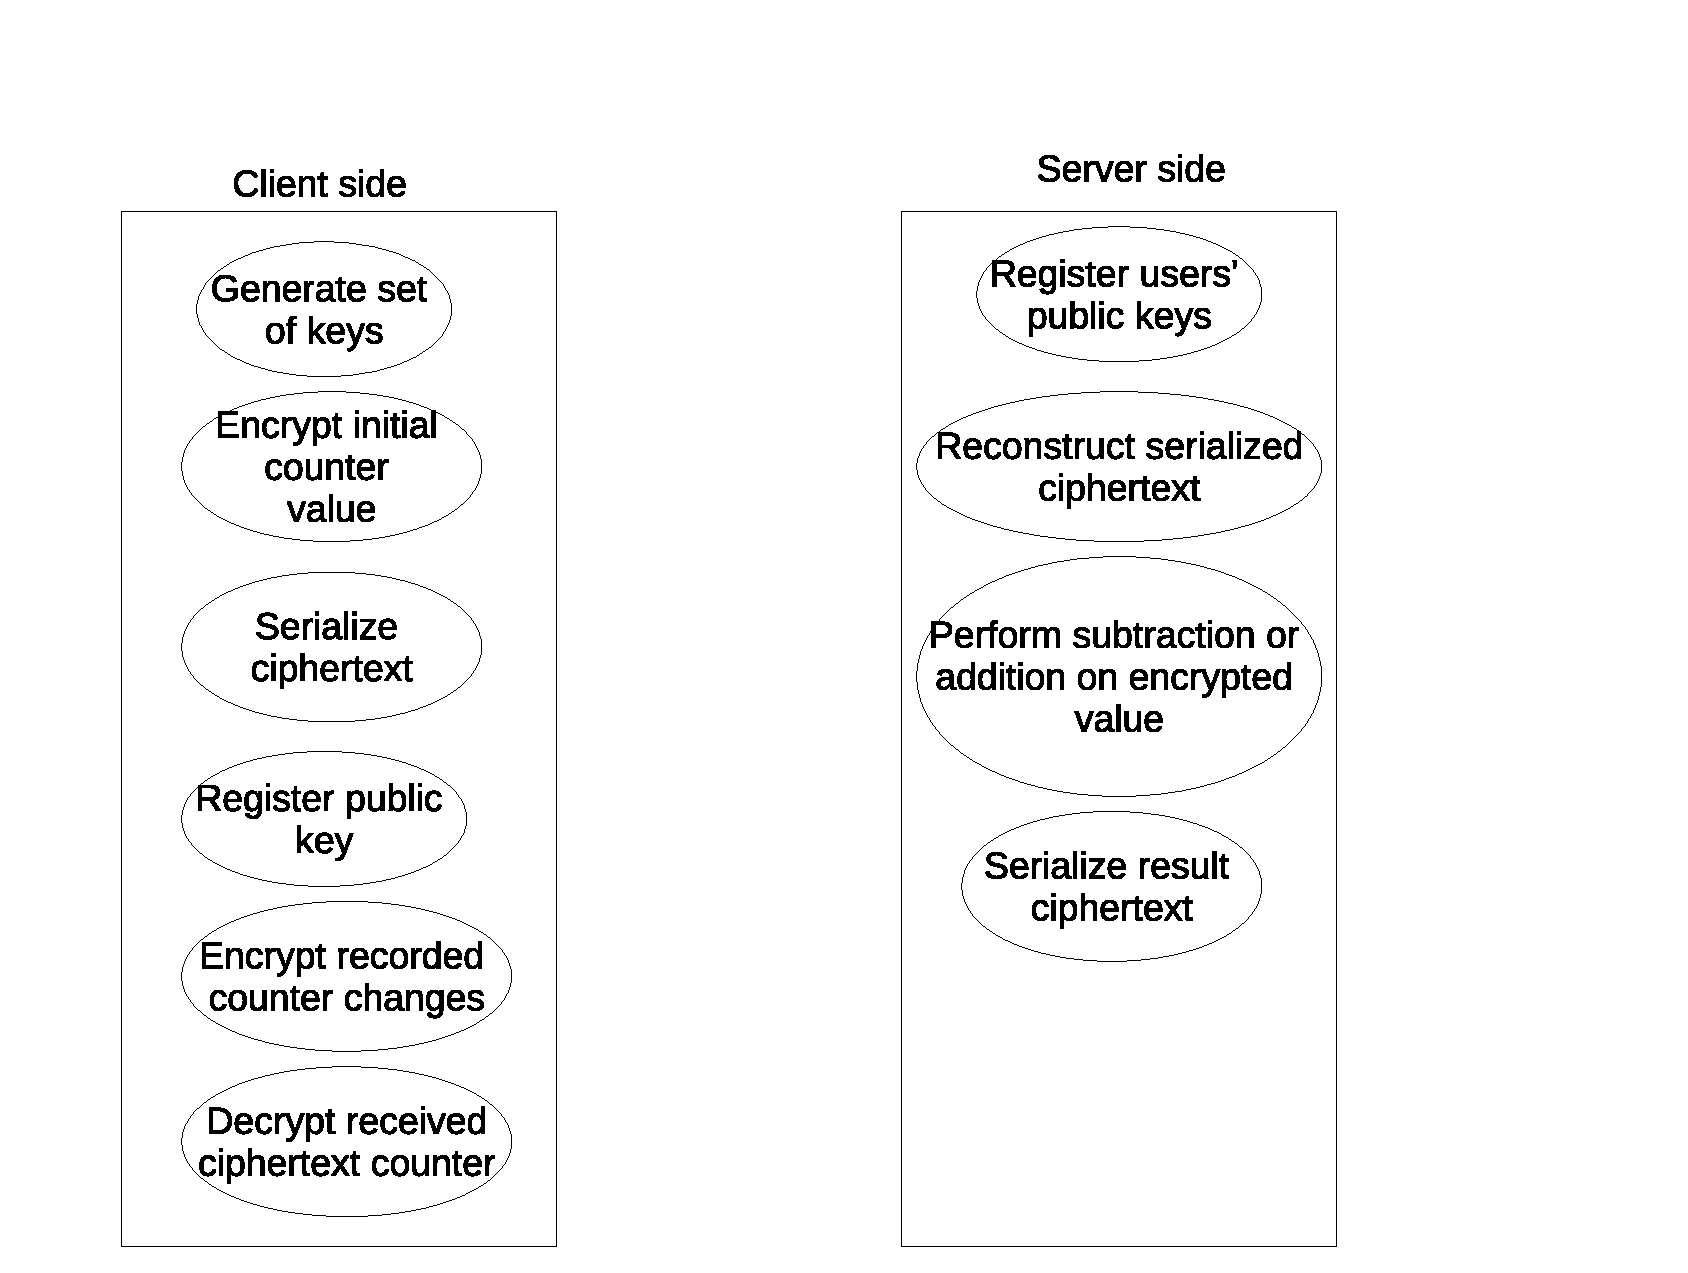
\includegraphics[scale=0.7]{clientserver}
  \caption{Architecture breakdown into client and server.}
\end{figure}

[ADD SEQUENCE DIAGRAM AND DESCRIPTION]

%\begin{figure}[h!]
%  \centering
%  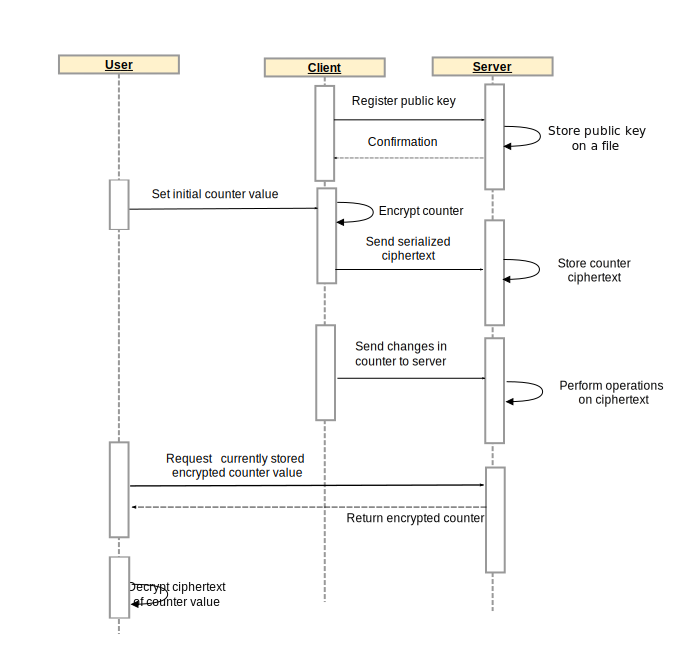
\includegraphics[scale=0.7]{counter}
%  \caption{Sequence diagram showing operation under normal conditions}
%\end{figure}

\textbf{Discussion}

The part of user registration is not part of the planned implementation itself, but it is recommended to consider how to handle different users. There might many more than a couple of households that make use of such a counting service. This is why each householder would have to register his public key and go through some kind of authentication mechanism every time they restart or download the counter data. It is especially important to take the appropriate measures so that somebody else does not reset the counter value of a household that is not theirs, because it would be chaotic when the householder looks at the counter and finds a value that does not represent reality.
To keep the registration under control, it might be ideal to keep a list of registered users either on a database or just a file for each household which would contain basic pieces of information such as an email address or username, along with the hash value of a password and the appropriate public key for the household that is being registered.

There were several problems at this stage that were directly related to the implementation. Th
e transmission of serialized data between the client and server was especially problematic. The early attempts at sending serialized data to the server were not quite successful. Many different kind of errors were found, and the most common one was related to memory allocation. After going through several trial and error attempts, it was found the errors started appearing as the message got larger. This seemed to be inevitable as the default settings of a TCP blocking socket were not adequate to send large pieces of data. 

After doing the right adjustments, the problem seemed to go away, except that \textit{the result was not quite as expected}. It was known inmediately that something was up with the received ciphertext, as it could not decrypt properly. It helped to look at the data that the server received, and it was quite evident that it was not complete. Indeed, only certain fragments of the ciphertext were received successfully, which led to an incorrect decryption. Several adjustments were made to the process of receiving data, so that a couple of control variables were used to keep in check how many bytes were being received. It was set so that it would only stop reading data from the client until all of the bytes had been read and assembled in a buffer. Both the functionalities of reading and writing the ciphertext on a socket were relatively more complicated considering that was done without the support of a framework that specialized on it.

In summary, a description of the case study was given, a solution based on homomorphic encryption was proposed to tackle the problem found in the case study, details of the HElib were discussed, and all of the relevant considerations pertaining to the implementation were explained. These considerations took on points such as the parameters and context, key generation and serialization, software architecture, transmission of serialized data, reconstruction of the ciphertext, and dealing with changes of the counter. 


\clearpage

%\include{caseStudy}
\chapter{Experiments and Results}
\label{results}

This section describes the design of the experiments related to the use of fully homomorphic encryption in HElib, as well as a summary of the results obtained. The objective of the experimental design was to test whether or not homomorphic encryption was practical enough to be applied in the cloud as a web application. The feasibility of application in the web depends heavily on the time required to perform homomorphic evaluations, which is affected by several factors. One of these main factors is the \emph{security parameter} $k$, which is a value closely related to the generation of public and private keys and how secure they are. The experimental design consists in changing the $k$ parameter to different values, as to see to what degree it has impact on the key generation, encryption, decryption and addition \emph{processing times}, as well as the \emph{size} of the resulting public key and ciphertext. Finally, the results obtained are presented and briefly discussed. 

\section{Setup}

The experiment is performed by running several iterations of the program that runs in the underlying client-server architecture, as to evaluate how the security parameter $k$ affects the time required for certain activities in the software, such as key generation, encryption, decryption, and homomorphic addition of ciphertext. Evidently, processing encrypted data homomorphically needs more computation than operating on the plaintext directly. The ratio between both computations is called the \emph{overhead}, and it is evaluated in terms of time. The security parameter $k$ is considered important because the value affects how secure the resulting keys and ciphertexts become, as well as the overhead of performing homomorphic evaluations. In the design document by Halevi and Shoup \cite{cryptoeprint:2014:106}, it does not specify to what degree changing the value of $k$ would make the cipher vulnerable to cryptanalysis or a brute-force attack; however, it does specify that the technique they propose uses a \emph{ciphertext packing} circuit that can be evaluated homomorphically in time $T \cdot $polylog($k$), which represents the overhead of the computation. Assuming the use of a circuit model of computation, the security parameter $k$ describes the width of the circuit being evaluated homomorphically.

To show how the $k$ security parameter affects the operation of the homomorphic encryption program, the experiment considers several arbitrarily chosen values, namely: 20, 40, 80, 100; where 80 is the default value found in the examples of the HElib. Each value is seen as a \emph{treatment} in the experimental design. For each treatment, the program is run through \textbf{20 iterations} of key generation, encryption, decryption and addition. 

In order to perform the necessary iterations, certain parts of the code from both the client and server sides were taken and adjusted, so that all the operations were performed on the same program. Consequently, overhead operation costs such as sending data between the client and server are not considered for this experiment.

When generating the public and private keys, all of the other parameters are kept \emph{intact}, so that it is only the $k$ value that gets changed. Consequently, the other mechanisms slightly vary because they make use of the previously generated public key.

It is important to consider that the experimentation was done on a notebook which had an AMD Elite A4-5150M processor. The processor is dual core and it runs at 2.7 GHz. Therefore, the results might differ depending on the processor used.% Implementation and experimentation of the client-server homomorphic counter solution were done on GNU Linux in the Xubuntu 14.04 distribution.

\section{Results}

The results are presented in Table \ref{tbl:results}, where the column represents the characteristic or attribute considered, such as the processing times and the size of the public key and ciphertext files measured in bytes. Consider that the values presented are the averages obtained from the set of iterations run.

\begin{table}[h]
  \caption{Experimental results}
  \label{tbl:results}
\begin{tabular}{lrrrrrr}
k   & Key Gen. & Key Size  & Encryption & Decryption & Addition & Ctext Size \\
40  & 13.130 s & 165.922 MB & 0.355 s    & 0.048 s    & 0.074 s  & 30.977 kB        \\
60  & 10.710 s & 91.635 MB  & 0.414 s    & 0.056 s    & 0.077 s  & 36.053 kB        \\
80  & 8.380 s  & 57.080 MB  & 0.642 s    & 0.057 s    & 0.082 s  & 37.745 kB        \\
100 & 9.529 s  & 35.453 MB  & 0.579 s    & 0.064 s    & 0.082 s  & 43.676 kB
\end{tabular}
\end{table}

In order to illustrate the differences observed, Figure \ref{fig:boxplot} depicts a box plot that shows the time required to generate the set of keys depending on the size of $k$. It was chosen not to plot the data pertaining to the rest of the attributes under experimentation, mostly because the differences observed were not significant.

\begin{figure}[h]
  \centerline{\includegraphics[height=7.5cm]{img/experimentplot}}
  \caption{Key generation time}
  \label{fig:boxplot}
\end{figure}


\section{Discussion}

The first characteristic that is being evaluated is the time needed to generate the set of public and private keys. Usually, the generation of keys is performed only once per user. Only if the private key were compromised, would the user create a new set of keys. Even though the highest average was 13 seconds for $k=40$, it is a relatively small amount of time. Directly linked to the generation of keys, the size of the key is considered relevant as well. Usually, the public key has to be shared with others, and in this particular case, the averages range between 165.92 MB for $k=40$  and 35.45 MB for $k=100$. The difference between both sizes is quite large, and even smallest key is significantly large by itself. Additionally, it is puzzling as to why the size of the public key is decreasing as the $k$ parameter gets larger. In cryptography, a larger $k$ usually implies a slowdown in the whole process, but in this case, it does quite the opposite, at least on the time needed for key generation.

%Preguntarte si los cambios son poco significativos

Regarding the encryption, decryption, and addition times, the average amount of time required is quite low, and it should not become a bottleneck even if many homomorphic evaluations are performed. Even though the encryption times are longer than the decryption times, none of them surpassed 1 second, which makes it quite acceptable in application. 

Perhaps the most important point to consider is the size of the generated ciphertexts. In the proposed architecture, a ciphertext is constantly sent to the server to perform operations and back to the client for decryption. According to the iterations run, the max average of the ciphertext size was found to be 43.67 kB for $k=100$, while smallest average was 30.99 kB for $k=40$. Looking at how the ciphertext sizes increases, it can be seen that it has a proportional relationship with the security parameter $k$. As $k$ gets larger, so does the size of the ciphertext. This would mean that higher security sacrifices storage, and consequently takes more time to transfer between the client and server.

Even assumming that a security parameter of $k=100$ is used, this shows that the size of the ciphertext is sufficiently small to be used in a web application hosted in the cloud. However, while the client-server architecture program was being developed, an average size of 74 MB per ciphertext was noted. At this time, it is not possible to recreate the scenario where ciphertexts of such a size were created, which leads to the impression that there is another factor not considered that accounts for the size of the ciphertext.

In conclusion, the aforementioned findings suggest that using HElib to apply homomorphic encryption in the cloud might indeed be feasible; however, as it has been noted, there are unknown circumstances that affect the size of the ciphertext. To the best of our knowledge, there is yet no way to predict the size of the ciphertext by using HElib. Therefore, if it is possible to keep the size of the ciphertext below 45kB, then it would certainly be feasible to take this solution to the cloud; otherwise, it would not be possible if each ciphertext had a size that exceeded several MB. Until these circumstances are made clear and evaluated properly, it is not possible at this time to show that using HElib to make use of homomorphic encryption in the cloud is indeed feasible. 

% Ver otra manera de poner la ultima oracion

\clearpage

%\include{existentes}

%\include{propuesta}
%\include{evaluacion}
\chapter{Conclusions}
\label{conclusions}

Se present\'{o} un enfoque para la detecci\'{o}n de documentos duplicados el cual est\'{a} basado en reconocimientos de entidades de un texto y aprendizaje computacional. Se trabaj\'{o} con los reportes ciudadanos del Centro de Integraci\'{o}n Ciudadana (CIC) como caso de estudio.

Otras cosas \ldots

\section{Comentarios finales}

Algo m\'{a}s que quieras decir \ldots

\section{Contribuciones}

Recordar cu\'{a}l fue tu contribuci\'{o}n.

\section{Trabajo a futuro}

Lo que falt\'{o} por hacer.

\clearpage


%\bibliographystyle{plain}
\bibliographystyle{estiloDeBibliografiaJorge}
\bibliography{bibliografia}

%\appendix
%\include{Apendice}

\printindex{}
\backmatter
\pagestyle{main}
%%Autobiografia

\chapter*{Ficha autobiogr�fica}
\chaptermark{Ficha autobiogr�fica}

\begin{center}
\autor

Candidato para el grado de \grado.

\uanl

\fime\bigskip

Tesis:
	
\begin{tabular}{p{11cm}}
	\centering
	\scshape{\large{\titulo}}
\end{tabular}
\end{center}

\bigskip

Nac\'{\i} el \ldots

\label{lastpage}


\end{document}
